\subsection{Computational Mesh Quality}
\label{ch3:sec:mesh_quality}

We now investigate the effectiveness of representing the entire computational mesh in the context of CFD.
To do this, we first use the OpenFOAM's mesh checking tool to evaluate the mesh quality after deformation.
Then simulations are performed on the generated meshes to analyze the effect of mesh reconstruction on aerodynamic performance.

\subsubsection{Quantitative Evaluations on Mesh Quality}
We use the 50 random NACA airfoils and 50 random non-NACA airfoils of any series from the UIUC airfoil dataset.
To study the role of $\cL_{reg}$ and AM Layer in preserving the mesh quality, all meshes are reconstructed from TM-A with the proposed model (Model \#4) and the three other variants (Model \#1-3):
\begin{itemize}
    \item \textbf{Model \#1} is trained without $\cL_{reg}$ and the AM Layer is not used.
    It serves as a baseline model.
    \item \textbf{Model \#2} is trained without $\cL_{reg}$, but the AM layer is used as post-processing.
    In this case, it takes more than $8,000$ iterations for Eq.\ref{ch3:eq:active_model_iteration} to converge on a 2D airfoil mesh.
    \item \textbf{Model \#3} uses $\cL_{reg}$ for training but the AM layer is not used.
    \item \textbf{Model \#4} uses both $\cL_{reg}$ for training and the AM layer for inference.
    The number of iteration can be largely reduced to $240$.
    Model \#4 is the default setting of the proposed model.
\end{itemize}

\begin{table}[!htbp]
  \centering
  \caption{\small Metrics used in the volumetric mesh quality check.}
    \begin{tabular}{crrrp{0.28\textwidth}}
    \hline
    \hline
    \textbf{issues} & \multicolumn{2}{c}{\textit{\textbf{errors}}} & \multicolumn{2}{c}{\textit{\textbf{qualities}}} \\
    \hline
    mesh   & \multicolumn{1}{l}{E1} & \multicolumn{1}{l}{number of negative volume cells} &        &  \\
    overlapping & \multicolumn{1}{l}{E2} & \multicolumn{1}{l}{number of incorrectly oriented faces} &        &  \\
    \hline
    skewness & \multicolumn{1}{l}{E3} & \multicolumn{1}{l}{number of highly skewed faces} & \multicolumn{1}{l}{Q1} & max skewness \\
    \hline
    \multirow{2}[2]{*}{orthogonality} & \multicolumn{1}{l}{E4} & \multicolumn{1}{l}{number of non-orthogonality errors} & \multicolumn{1}{l}{Q2} & max non-orthogonality \\
           &        &        & \multicolumn{1}{l}{Q3} & mean non-orthogonality \\
           &        &        & \multicolumn{1}{l}{Q4} & number of severely non-orthogonal faces  (> $70^\circ$)\\
    \hline
    \hline
    \end{tabular}%
    \label{ch3:tab:mesh_check_notions}
\end{table}%

\begin{table}[!htbp]
  \centering
  \caption{\small Average mesh quality evaluation results over 100 random airfoils.}
    \begin{adjustbox}{max width=\textwidth}
    \begin{tabular}{cccccccccc}
    \hline
    \hline
    airfoils & models & E1     & E2     & E3     & E4     & Q1     & Q2     & Q3     & Q4 \\
    \hline
    \multirow{4}[2]{*}{NACA} & \#1    & 364.74  & 2245.54  & 535.40  & 476.82  & 12348.725  & 178.861  & 12.607  & 277.66\\
           & \#2    & 0.00   & 0.08   & 0.02   & 0.06   & 0.771  & 49.424  & 9.017  & 2.40  \\
           & \#3    & 0.00   & 534.12  & 3.86   & 109.96  & 480.298  & 137.272  & 9.852  & 44.42  \\
           & \#4    & 0.00   & 0.00   & 0.00   & 0.00   & 0.543  & 42.668  & 9.020  & 6.30  \\
    \hline
    \multirow{4}[2]{*}{non-NACA} & \#1    & 435.98  & 2657.66  & 513.80  & 572.02  & 2031.345  & 179.113  & 13.675  & 353.48\\
           & \#2    & 0.00   & 0.30   & 0.06   & 0.08   & 0.803  & 51.442  & 9.100  & 10.26  \\
           & \#3    & 0.00   & 65.32  & 0.40   & 10.92  & 11.222  & 101.035  & 8.646  & 16.52  \\
           & \#4    & 0.00   & 0.00   & 0.00   & 0.00   & 0.486  & 36.073  & 8.292  & 0.00 \\
    \hline
    \multirow{4}[2]{*}{overall} & \#1    & 400.36  & 2451.60  & 524.60  & 524.42  & 7190.035  & 178.987  & 13.141  & 315.57 \\
           & \#2    & 0.00   & 0.19   & 0.04   & 0.07   & 0.787  & 50.433  & 9.059  & 6.33  \\
           & \#3    & 0.00   & 299.72  & 2.13   & 60.44  & 245.760  & 119.154  & 9.249  & 30.47  \\
           & \#4    & 0.00   & 0.00   & 0.00   & 0.00   & 0.514  & 39.371  & 8.656  & 3.15  \\
    \hline
    NACA-  & \multirow{2}[2]{*}{TM-A} & \multirow{2}[2]{*}{0.00 } & \multirow{2}[2]{*}{0.00 } & \multirow{2}[2]{*}{0.00 } & \multirow{2}[2]{*}{0.00 } & \multirow{2}[2]{*}{0.486 } & \multirow{2}[2]{*}{30.144 } & \multirow{2}[2]{*}{7.520 } & \multirow{2}[2]{*}{0.00 } \\
    0012   &    &        &        &        &        &        &        &        &  \\
    \hline
    \hline
    \end{tabular}%
    \end{adjustbox}

  \label{ch3:tab:mesh_check_results}%
\end{table}%

OpenFOAM's \textit{checkMesh} command  is used for evaluation.
This tool generates a short report that contains several quantitative results.
We divide these statistics into two categories, i.e. \textit{errors} and \textit{qualities}.
Any occurrence of \textit{errors} in the report indicate existed fatal issues that impair the simulation's correctness.
The \textit{quality} results are geometric criteria of the mesh that affect the stability, convergence speed and residual control of simulations.
We use 8 measurements in total for a comprehensive evaluation.
Tab.\ref{ch3:tab:mesh_check_notions} explains the meanings of all metrics and lower values indicate better mesh qualities.
The evaluation results are compared with the template mesh quality in Tab.\ref{ch3:tab:mesh_check_results}.
Several qualitative comparisons are shown in Fig.\ref{ch3:fig:exp_mesh_quality}.

\begin{figure}[!htb]
	\begin{center}
		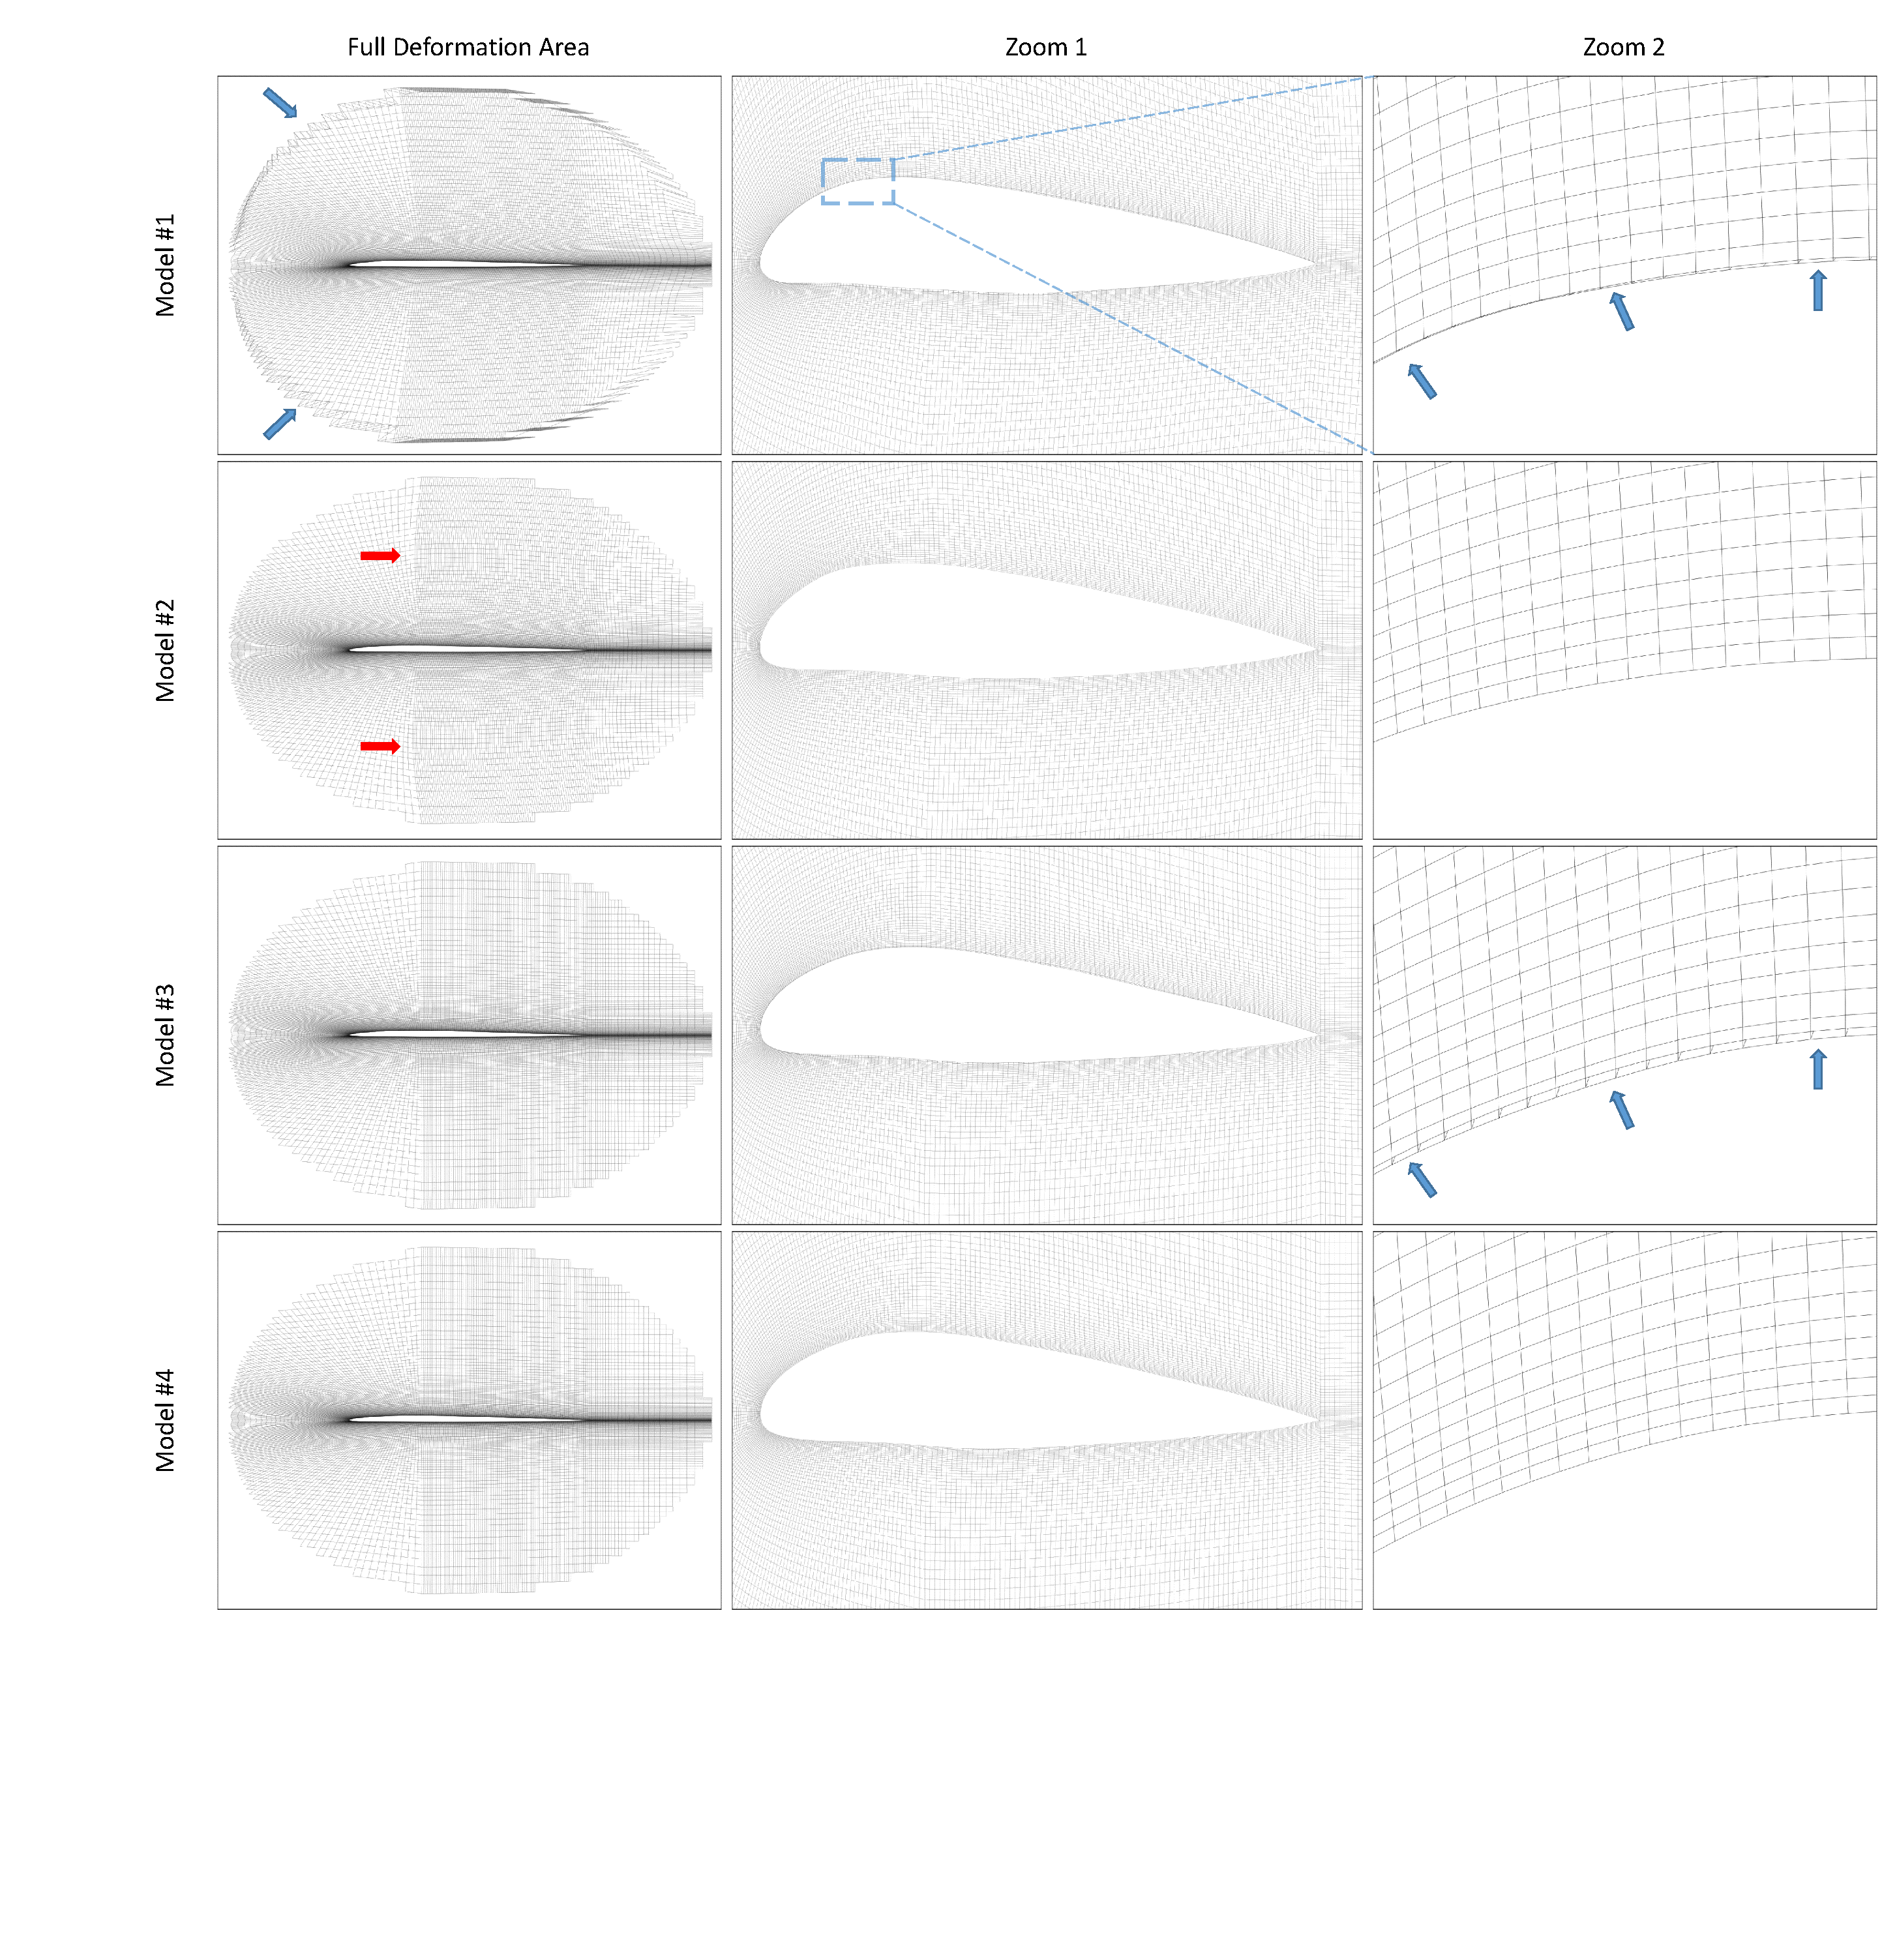
\includegraphics[width=1\linewidth]{chapter3/tex/figures/experiment/mesh_quality_ablation.pdf}
	\end{center}
	\caption{
		\small Illustrations of NACA-24109's meshes generated by Model \#1-4. Blue and red arrows highlight the overlapping and non-orthogonal issues.
	}
	\label{ch3:fig:exp_mesh_quality}
\end{figure}

Model \#1 has no guarantee on the mesh quality without any explicit constrains or post-processing.
The results of Model \#2 show that the AM layer solves almost all the overlapping issues and other severe errors, but some global non-orthogonality remains.
Using $\cL_{reg}$ for training while removing the AM layer as in Model \#3 removes the large mesh distortion near the boundary of the deformation area, as shown in Fig.\ref{ch3:fig:exp_mesh_quality}, but the overlapping issue near the object surface is not totally solved.
However, the combination of $\cL_{reg}$ and AM layer as in Model \#4 is most effective.
Meanwhile, Model \#4 works consistently well on NACA and non-NACA airfoils, which demonstrates its robust generalization ability.
Compared with the NACA-0012 template mesh TM-A, Model \#4 produces meshes without errors and with the same order of magnitude for quality metrics Q1-Q4. It explains the proposed model with $\cL_{reg}$ and the AM layer is suitable for CFD, as it produces meshes of similar quality as a handcrafted one, in an automated manner.

\subsubsection{Case Studies on Simulations}
\label{ch3:sec:simulation}

In this section, we validate the quality of our generated meshes when used to simulate 2D airfoil dynamics. To this end, we compare simulation results obtained using our meshes with experimental data from the UIUC Low Speed Airfoil Data~\cite{aa.Selig1995,aa.Selig1996b,aa.Lyon1998, aa.Williamson2012} and the CFD data generated automatically by the VLab computational framework \cite{aa.Chappin2010,aa.Viola2018}.

\begin{figure}[!htb]
	\begin{center}
		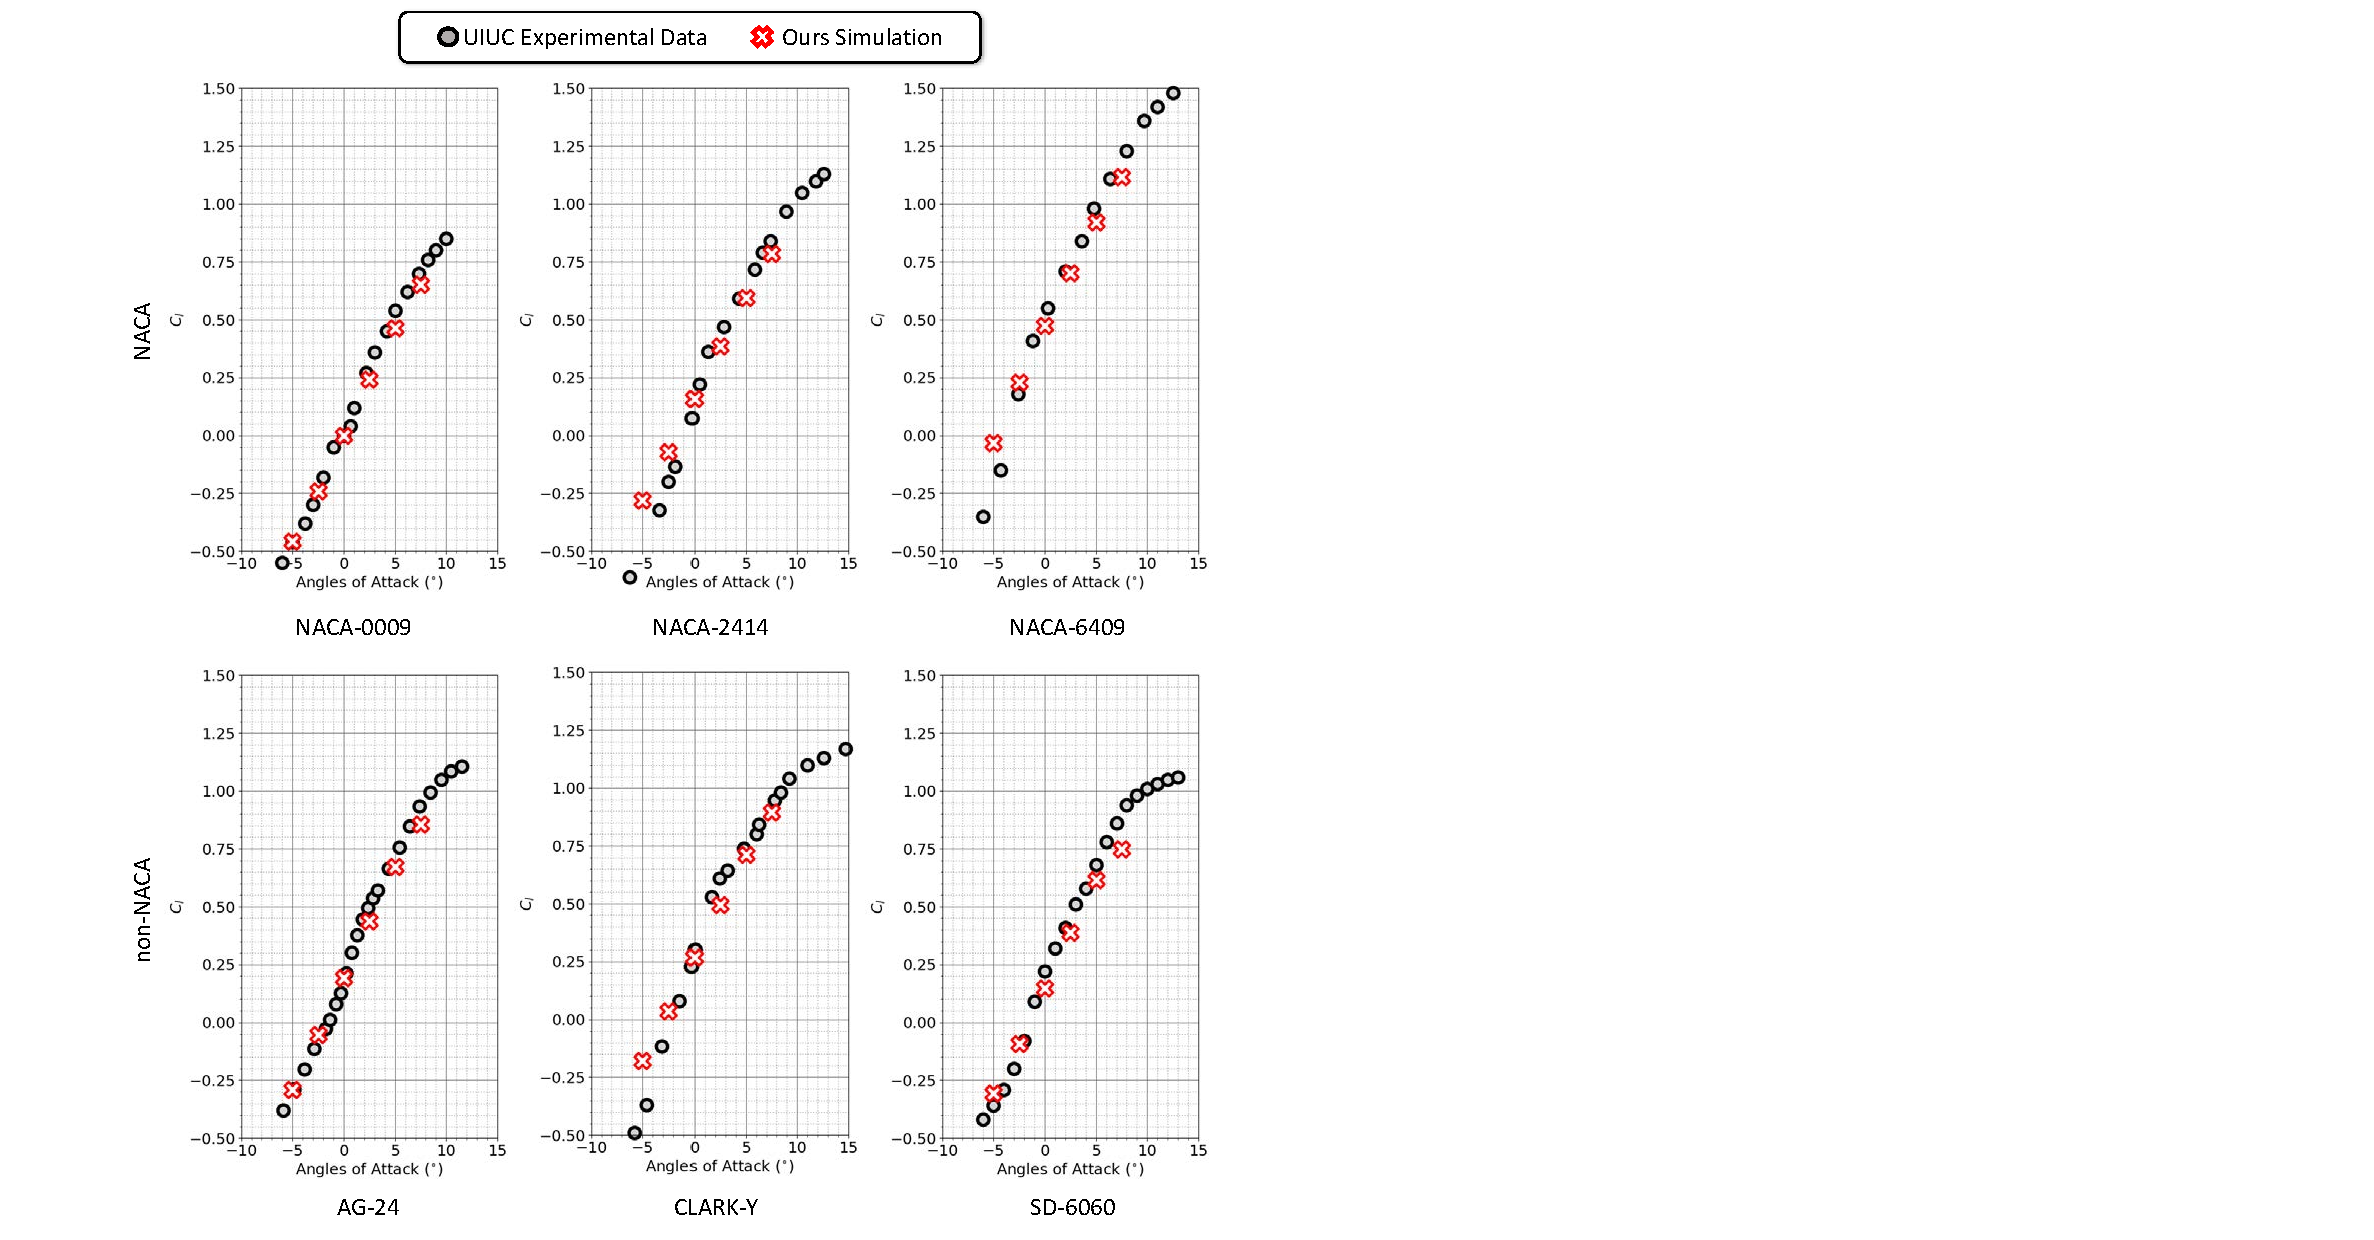
\includegraphics[width=1\linewidth]{chapter3/tex/figures/experiment/simulation_UIUC.pdf}
	\end{center}
	\caption{
		\small Comparisons between the simulation results on deformed meshes and the UIUC's experimental data.
		%Both NACA and non-NACA airfoils are tested.
	}
	\label{ch3:fig:exp_simulation_UIUC}
\end{figure}

\begin{figure}[htb]
	\begin{center}
		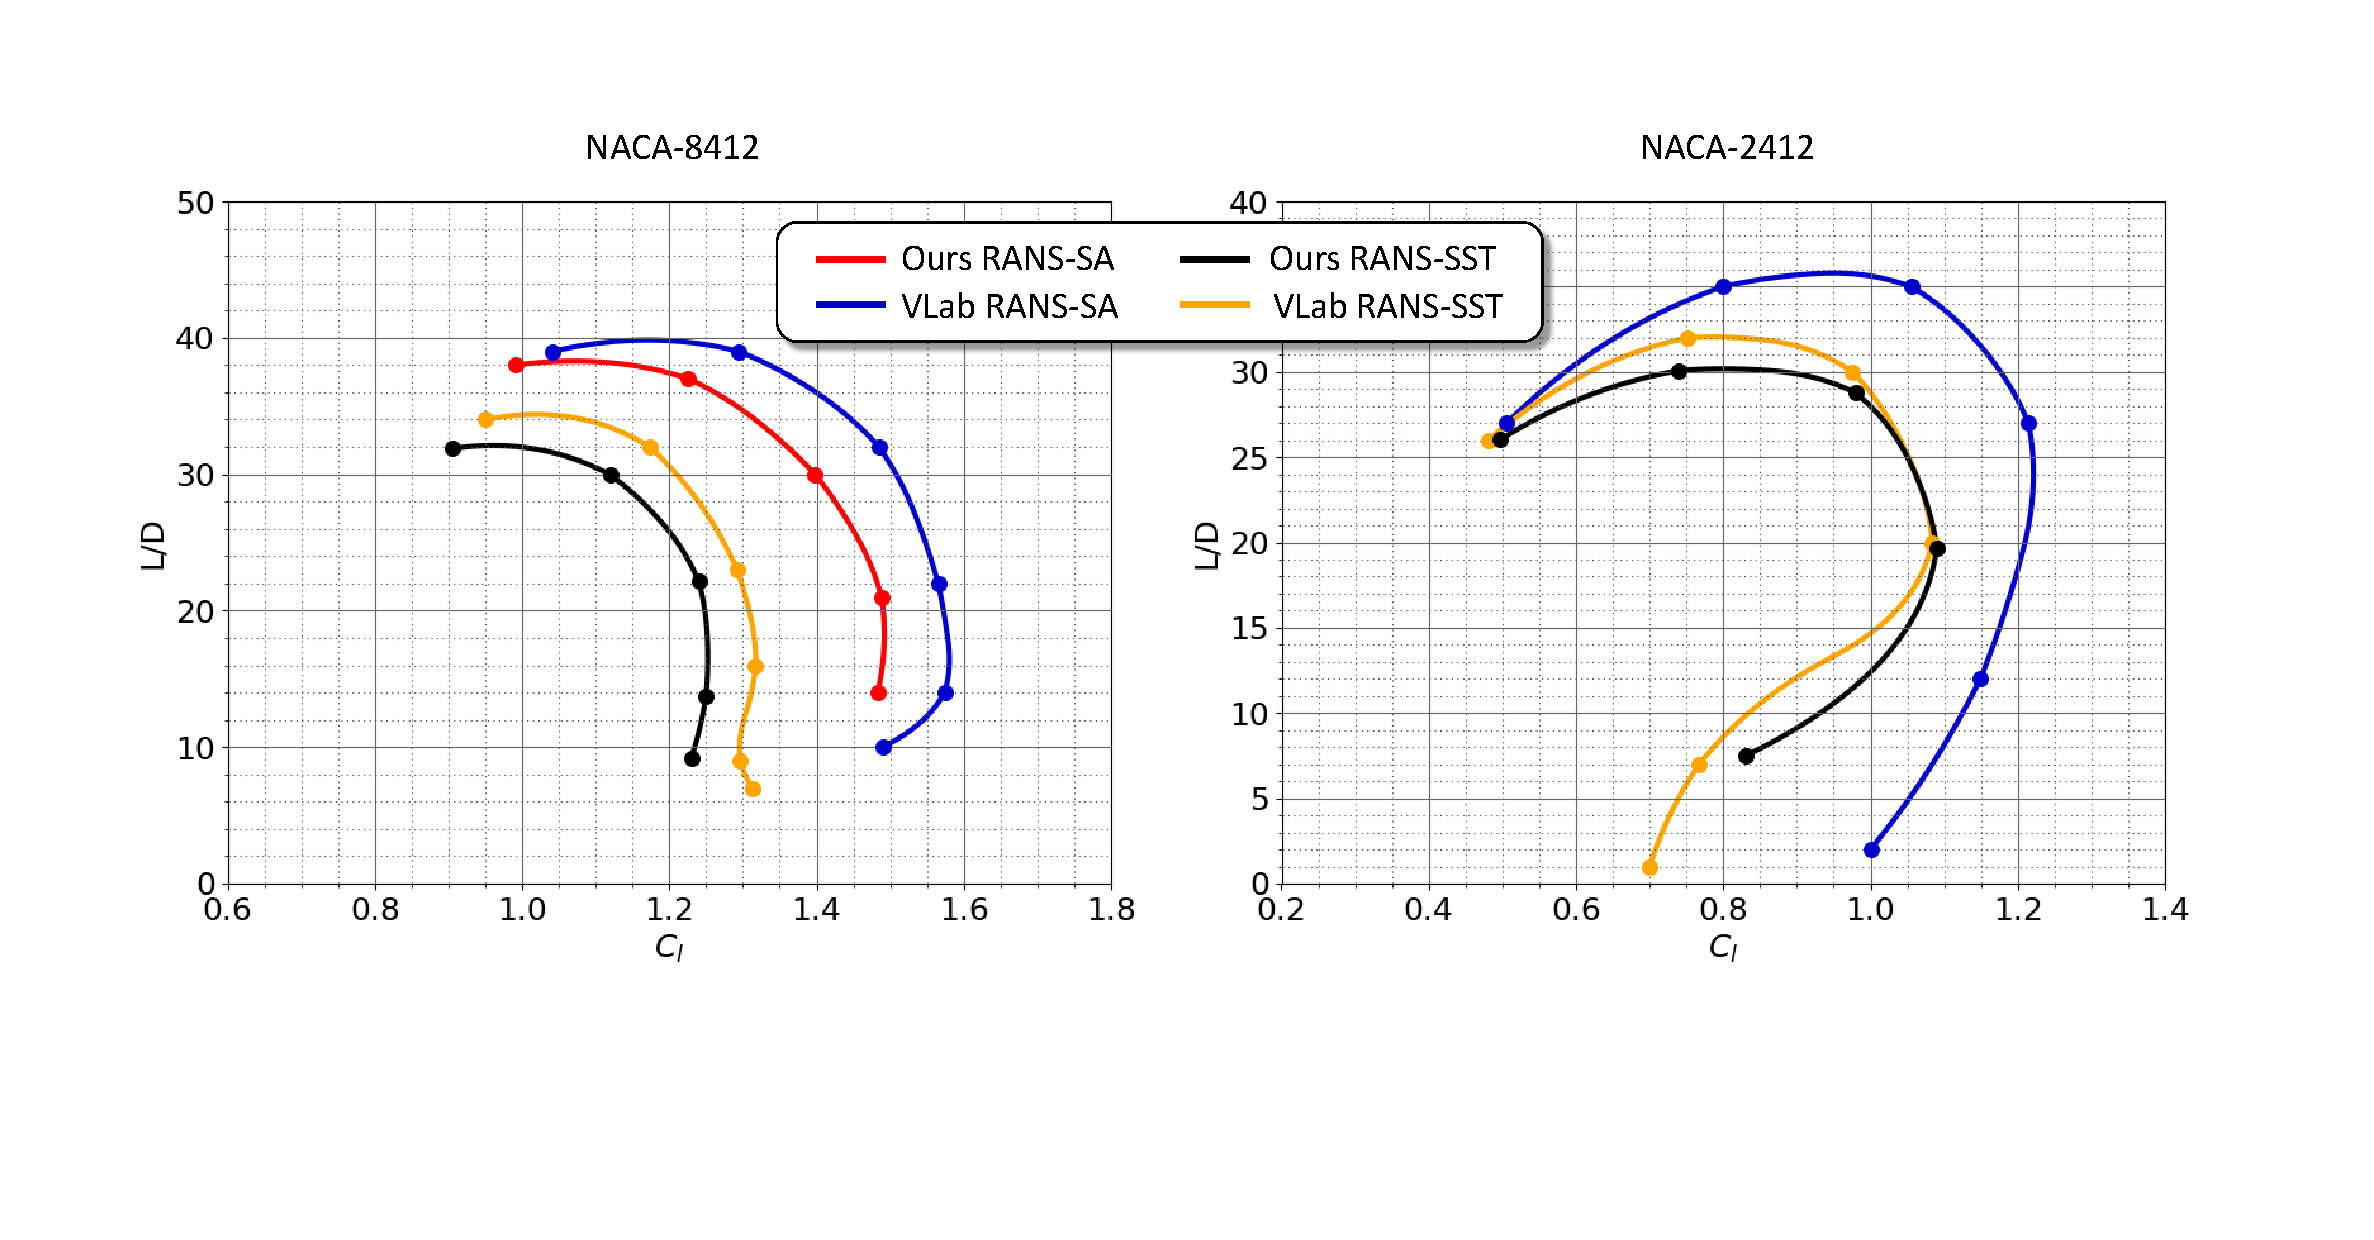
\includegraphics[width=1\linewidth]{chapter3/tex/figures/experiment/simulation_supaero.pdf}
	\end{center}
	\caption{
		\small Comparisons between the simulation results on deformed meshes and VLab reference data.
	}
	\label{ch3:fig:exp_simulation_supaero}
\end{figure}

The UIUC Low Speed Airfoil Data features airfoil tests at low-Reynold numbers in the UIUC wind tunnel. 
This dataset contains testing results on various airfoils.
We select the data of lift coefficients at $Re=10^5$ of three NACA airfoils (i.e. NACA-0009 / 2414 / 6409) and three non-NACA airfoils (i.e. AG-24, ClarkY and SD-6060) as references.

The VLab data is composed of high-fidelity numerical simulations created by the computational framework VLab \cite{aa.Chappin2010,aa.Viola2018}. It uses parametric hybrid meshes and ANSYS\textsuperscript{\textregistered} Fluent\textsuperscript{\textregistered} to provide CFD of various shapes in an automatic way.% has been used. %Meshes are generated with VLab with $y^+<1$ to avoid the use of wall models.
We refer to NACA-2412 and NACA-8412.

% simulation setups, need discussion
For the UIUC Low Speed dataset comparisons, the simulations were performed by running OpenFOAM on computational meshes generated from TM-A for the reference airfoils. We use the RANS solver coupled with the \textit{k}-omega-SST turbulence model \cite{aa.Menter1993} at $Re=10^5$.
For the VLab data comparison, meshes for both airfoils are generated based on TM-B. The CFD meshes are then used in VLab's solver for RANS simulations at $Re=10^6$. Both the Spalart–Allmaras \cite{aa.Spalart1992} and the \textit{k}-omega-SST turbulence models are used for the respective simulations, allowing for the study of mesh effects by comparing discrepancies caused by different meshes and turbulence models.

Fig.\ref{ch3:fig:exp_simulation_UIUC} shows our simulation data at AoAs of $-5^\circ$, $-2.5^\circ$, $0^\circ$, $2.5^\circ$, $5^\circ$ and $7.5^\circ$.
The simulated lift coefficients fit well with the wind tunnel experimental data.
The averaged y+ values of these cases range from $1.94$ to $2.49$, and the mean y+ when simulating on TM-A is $2.19$.
In Fig.\ref{ch3:fig:exp_simulation_supaero}, the simulated results resolve the trend of lift-drag ratio with the changes of lift coefficients.
The averaged y+, for example the one of NACA-2412, is $1.47$ while the y+ of simulating on TM-B is $1.42$.
These results confirm that the deformed meshes decoded by the proposed model have adequate quality for CFD simulations. The proposed mesh model well preserve the boundary layer qualities given both template meshes,  and the errors have minimal effects on simulation results.